\documentclass[10pt]{article}
\usepackage{graphicx} % Required for inserting images
\usepackage{subcaption}
\usepackage{float}
\usepackage[T1]{fontenc}
\usepackage[utf8]{inputenc}
\usepackage{lmodern}
\usepackage[english]{babel}
\usepackage[autostyle]{csquotes}
\usepackage[mode=buildnew]{standalone}
\usepackage{tikz}
\usetikzlibrary{positioning, fit, shapes.geometric, calc}

\usepackage{comment}

\usepackage[backend=biber,style=authoryear]{biblatex}
\addbibresource{bibliography.bib}

\title{Image Classification on Satellite Imagery For Sustainable Water Harvesting Placement in Indigenous Communities of Northern Tanzania}
\author{Roshan Taneja, Yuvraj Taneja}
\date{\today}

\begin{document}

\maketitle

\begin{abstract}

In the remote regions of Northern Tanzania, women and children of the Maasai Tribe walk nine hours a day to collect water for their families. Over four years, the collaborative efforts with the Maasai communities have led to the installation of four water harvesting units, enhancing the local socio-economic conditions by facilitating educational opportunities and economic pursuits for over 4,500 individuals within a 10-mile radius.

This project presents a novel approach to addressing this issue by integrating satellite data and image classification to identify densely populated areas marked by uniquely shaped Maasai homes lacking a water supply and planning the best placement of rainwater harvesting units. The backbone of this project was developing an image classification model trained on 10,000 hand-selected satellite image samples of Bomas. This model generated a density heat map, enabling the strategic placement of water harvesting units in the most critical locations to maximize impact.

Our findings underscore the potential of satellite technology in humanitarian interventions, particularly in harder-to-reach areas where traditional surveying and data collection techniques are impractical.
    
\end{abstract}

% ------------------------------------------------------------------------------------

\section{Introduction}

\subsection{Background and Context}

According to the United Nations, one in four people cannot access clean water (\autocite{United_Nations}). One such community is the Maasai in the Monduli District of Tanzania. They walk over nine hours daily to fetch water and face climate change and land deforestation challenges (\autocite{taneja2024impact}). Floods and droughts are more frequent and severe, and traditional water sources, such as rivers and springs, dry up. Annual rainfall in Tanzania is equal to or higher than in the US, yet they face challenges in accessing water. The community has been deploying water harvesting units along the main highway, which currently helps less than 4000 people, but only during the rainy season. The impact of even one water harvesting unit has been validated. The challenge is that over 30,000-40,000 Maasai live across hundreds of square miles without highways and infrastructure like electricity or water. A better technique needs to be identified to assess the living locations, the density, and pick the right water harvesting solution that balances cost, ease of deployment, and sustainability. This paper takes the first step in identifying the living locations across hundreds of square miles using satellite images, machine learning, and image classification models. If this approach has high precision, it can be expanded to many regions for water resource planning and management opportunities.  There is a need for sustainable water management solutions to support communities like the Maasai and other areas of Africa.

\begin{figure} [H]
    \centering
    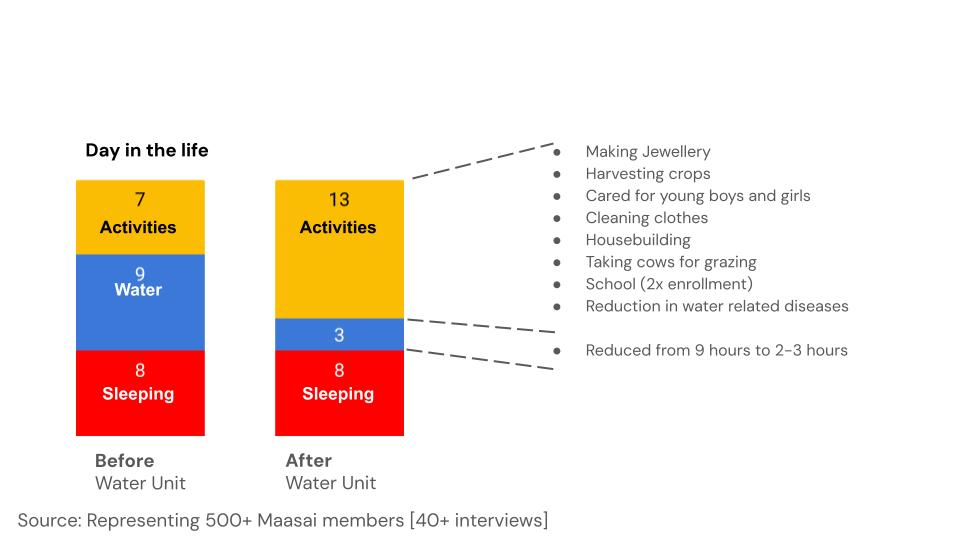
\includegraphics[width=1\linewidth]{images/beforeandafterwhu.jpg}
    \caption{Before and after the Water Harvesting Unit: Doubled the time spent on economic, social, and agricultural activities}
    \label{fig:bef_aft_results}
\end{figure}

The first water harvesting unit of 100K liters had a direct impact on the community. Specifically, kids have started coming to school more often and there is higher enrollment of students. Women have seen reduced time spent walking to fetch water and are using the extra time for social, agriculture and economic activities. Reduced walking from nine hours a day to two hours a day (Fig~\ref{fig:bef_aft_results}). 

Given the impact, multiple additional projects have been executed include deploying a 30+K liter solutions serving the Nanja village and a water filtration system in Engirgiri that makes water collected in man-made pond that catches rainwater clean for use by the local community of Maasai.


% ------------------------------------------------------------------------------------


\subsection{Problem Statement and Rationale}

% This isn't a problem statement

To support water harvesting solutions for 30,000-50,000 Maasai, identifying the best places to locate them across 300-500 square miles was the primary concern. The best water harvesting solutions would ideally be based on the population's density distribution, and nearby available water resources. However, the government does not provide accessible maps of the Maasai's location. To design and plan solutions at scale,satellite images and image classification helped to create a population map and validate the maps with local community involvement. The next step would be identifying the best locations for placing the water harvesting solutions.



% In Northern Tanzania, the Maasai community faces a severe challenge in accessing clean and safe water due to the arid climate and inadequate water infrastructure. This region, spanning thousands of square miles, predominantly relies on traditional water sources like rivers and springs, which are increasingly unreliable due to climate change and government intervention. The unique living structures of the Maasai, known as "bomas," are typically circular or oval enclosures made from thorny bushes and are difficult to detect using standard remote sensing techniques. These bomas, housing between 10 to 100 individuals, often do not have direct access to water sources, exacerbating the daily struggle for water.

% To address this critical issue, our project leverages satellite data to detect these uniquely shaped Bomas across extensive areas. By using advanced image classification techniques, we can identify densely populated regions lacking sufficient water access. The data source includes high-resolution satellite imagery analyzed through a custom-developed image classification model trained on 10,000 hand-selected images of Maasai homes.

%The solutions proposed aim to optimize the placement of water harvesting units based on the identified needs and local geographical conditions. The options for enhancing water accessibility include large units for housing groups, such as installing communal rainwater harvesting units with capacities of 100,000 liters to serve large groups of bomas, ensuring a continuous water supply for several days. Small Units on a Per-Boma Basis: Smaller, individual water collection systems for single bomas or small clusters provide a more personalized water management approach.Man-made Ponds and Dams: Creating larger-scale rainwater collection systems such as ponds or dams to benefit entire communities, especially in more densely populated areas.

% This comprehensive approach aims to provide immediate relief from water scarcity and contribute to the long-term sustainability of the Maasai way of life by integrating modern technology with traditional living patterns. The expected outcomes include reduced time spent collecting water, improved health and hygiene, and enhanced economic and educational opportunities for the community.


% ------------------------------------------------------------------------------------


\subsection{Scope and Limitations}

The study will be limited to a selected area of about 250 sq. miles. In addition, limited modifications will be made to the base computer vision algorithm. These limitations enable a rapid iterative process to be used to finalize the correct training data and algorithms. There are also other limitations in the data being used.

\subsubsection{Unique Structure and Materials of Bomas}

\begin{figure} [H]
    \centering
    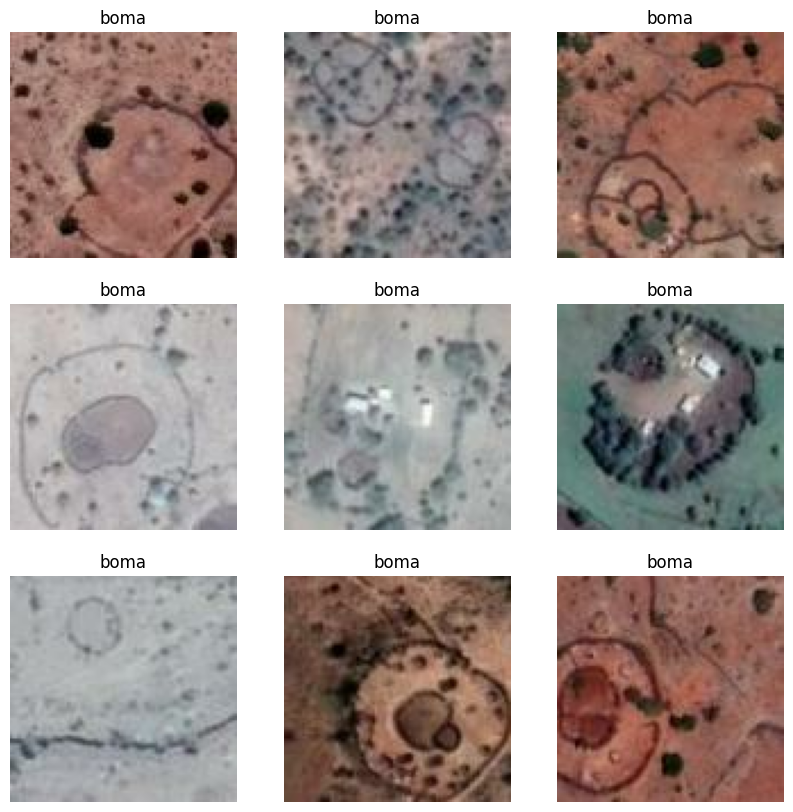
\includegraphics[width=0.8\linewidth]{images/types of bomas.png}
    \caption{Example of Variation in Landscape, Vegetation and Structure}
    \label{fig:types_of_bomas}
\end{figure}

Due to their polygamous nature, familial groups live together in large units called "Bomas." 

A Boma is a unique structure that is difficult to classify. There is no precise size to a Boma, but it usually consists of multiple small huts, a section for keeping goats and cows safe at night. There are a few characteristics that define a Boma. An outer barrier, usually made from rough bushes. Inside, there may be trees or other structures, such as shelters. At the center will be a smaller circle, also created with bushes, where cattle stay. These Bomas can house 10 to 50 people and sometimes be squares or other shapes, even open ones. Families who own cattle create an inner or outer circle or circles with other things, such as trees. Another issue is the contrast of the bushes with the environment, sometimes not showing up. (Fig~\ref{fig:types_of_bomas})

\subsubsection{Literature Review}

This section reviews related works for deep learning methods for classifying remote sensing satellite images. Classification of remote sensing images using machine learning is challenging because images are characterized by multi-resolution, heterogeneous appearance, and multi-spectral channels. Convolutional neural networks have a lot of limitations, including quality assurance of inputs, false negatives, overfitting, and the complicated nature of hyperparameters. Recent remote sensing and deep learning research has explored various methods for analyzing and classifying satellite images. Three research papers are included below to explain the range of methods but are not comprehensive.

(\autocite{richardson2023dense}) focused on mapping lichen to support caribou conservation efforts using machine learning models. They trained a dense neural network to map lichen coverage, achieving an accuracy based on Sentinel-2 imagery and UAV data from 20 sites in Québec and Labrador. The data was processed using Pix4D and Google Earth Engine. The model used 10-meter resolution maps and minimized spatial autocorrelation with a blocking strategy. The best-performing model, a dense neural network with an R² of 0.76, was trained with the Adam optimizer, and overfitting was avoided with early stopping.

(\autocite{liu2024stransu2net}) proposed STransU2Net for building extraction from satellite imagery using a hybrid approach that combines Convolutional Neural Networks (CNN) and Transformer architectures. CNNs are effective for capturing local features but struggle with more significant buildings, while Transformers are better at capturing global context but not small buildings. STransU2Net overcomes these limitations by integrating both models and adding advanced features like Bottleneck Pooling Blocks (BPB) and Channel And Spatial Attention Blocks (CSAB) to preserve edge information and focus on essential features. The model was trained on two datasets, achieving impressive results, with 91.04\% IoU on the Aerial imagery dataset and 59.09\% IoU on the Satellite II dataset. Combining local feature extraction (CNN) and global context modeling (Transformer) made building segmentation tasks more efficient and accurate.

(\autocite{2010.06497}) explored deep learning for satellite image classification, specifically using Convolutional Neural Networks (CNNs) to detect objects in satellite imagery. Their system was tested on the IARPA Functional Map of the World (fMoW) dataset, which includes large-scale, multi-spectral satellite images. The model successfully classified objects into 63 categories with 83\% accuracy and an F1 score of 0.797. The study highlighted challenges in preprocessing satellite images, such as cloud cover, resizing that lost essential details, and the limitations of labeled satellite datasets. By integrating metadata with image features, the system improved accuracy and managed false detections effectively.

The above techniques were not implemented explicitly. This project used data augmentation of the training data, and the method is detailed in the following sections.


\subsubsection{Image Processing Pipeline}

\begin{figure} [H]
    \centering
    \includestandalone[width=1\textwidth]{pipeline}
    \caption{Image Processing Pipeline}
    \label{fig:pipeline}
\end{figure}

The image processing pipeline illustrated in the diagram (Fig~\ref{fig:pipeline}) is centered around detecting and clustering dwellings from satellite image data to support resource provisioning. The process begins with a Satellite Image Database (Fig~\ref{fig:pipeline}:05) that stores raw satellite images (Fig~\ref{fig:pipeline}:03) and associated metadata (Fig~\ref{fig:pipeline}:04). These images are divided into training data (Fig~\ref{fig:pipeline}:02A) and validation data (Fig~\ref{fig:pipeline}:02B), which are processed by an Input Processor (Fig~\ref{fig:pipeline}:10) to prepare the dataset for model training. The Model Generator (Fig~\ref{fig:pipeline}:11) creates a detection model (Fig~\ref{fig:pipeline}:12) using parameters (Fig~\ref{fig:pipeline}:21) and weights (Fig~\ref{fig:pipeline}:22) stored in the Model Database (Fig~\ref{fig:pipeline}:20). This trained model is then used to analyze the images and extract dwelling locations (Fig~\ref{fig:pipeline}:41), including associated geographical data (Fig~\ref{fig:pipeline}:42) and timestamps (Fig~\ref{fig:pipeline}:43).

Once dwelling locations are identified, the data is further refined through a Clustering Process (Fig~\ref{fig:pipeline}:16) to group dwellings into clusters (Fig~\ref{fig:pipeline}:45), which are stored in a Dwelling Database (Fig~\ref{fig:pipeline}:40). The clustering process helps identify patterns or group dwellings based on proximity or other relevant factors, which can be analyzed temporally using the Temporal Analyzer (Fig~\ref{fig:pipeline}:54). This clustered information is then utilized by the Resource Provisioning Unit (Fig~\ref{fig:pipeline}:50), which includes components like a Water Consumption Estimator (Fig~\ref{fig:pipeline}:51) and a Water Unit Calculator (Fig~\ref{fig:pipeline}:52). These tools enable precise calculation and allocation of water resources to dwelling clusters, guided by resource instructions (Fig~\ref{fig:pipeline}:44) considering their specific geographical and temporal requirements. The pipeline is designed for efficient resource allocation by leveraging satellite imagery and advanced machine learning models.

\subsubsection{Techniques Considered}

In evaluating three different methods for this project, the computer visions considered were YOLOv7, OpenCV, and TensorFlow. YOLOv7, though highly optimized for speed and accuracy with minimal background detection errors, presented significant challenges. It proved difficult to integrate with Jupyter notebooks(\autocite{s23135849}). It performed inadequately with objects of varying sizes and shapes—critical for this project—and suffered from limited community support(\autocite{IJERTV10IS060287}), maintained by a small team. While boasting extensive community support and customizable settings, OpenCV was deemed overly complex, featuring a steep learning curve(\autocite{9174593}).

Conversely, TensorFlow appeared as the optimal choice, balancing accessibility as an open-source tool and compatibility with Python and JavaScript, which is crucial for integrating with Google Earth Engine (GEE).
Despite its higher resource consumption and slower performance, TensorFlow's regular updates and new features make it the most suitable framework. It provides the necessary tools and support for successful project execution.

\subsection{Objectives}

This research project aims to optimize the placement of water harvesting solutions based on population density and natural water sources. A population density map would be generated, using satellite data to detect these uniquely shaped Bomas across selected regions. This data will help identify critical locations for deploying the appropriate water solutions. The options for enhancing water accessibility include large units for housing groups, such as installing communal rainwater harvesting units to serve large groups of Bomas and creating larger-scale rainwater collection systems, such as ponds or dams, to benefit entire communities, especially in more densely populated areas.

% ------------------------------------------------------------------------------------

\section{Methods}
\label{methods}

\subsection{Data}

Two different sources were considered for the training data. One was the Copernicus Institute website for the Copernicus Satellites and Google Earth Engine (GEE). GEE was the better option because writing a script to generate the training data from just a few points on a map was easier.

\subsubsection{Collection}

2000 photos of Bomas and 500 photos of the environment (Omits a Boma) was the first iteration of training data. The accuracy was around 30\%, far below the required standards. The model needed help with a few problems. First, The color of the Boma circle blended in too well with the environment. Second, There wasn’t enough data to train the AI.


\subsubsection{Augmentation}

A key insight employed was the fact that these images could be superimposed, meaning they could be rotated and flipped to create more training data for the model. Using this new information, 6,000 more photos of Bomas and 1500 more images of the environment were generated. With this new model trained at 10,000 images, the accuracy skyrocketed to 93\%. Because these "Bomas" are often disguised and varied, more training would not increase the accuracy further. The model plateaus with the current constitution at a certain point due to the extreme shape, color, and size variation. Toggling with filters, cropping, grayscale, or increasing the contrast did not impact the accuracy. Perhaps more fine-tuning is necessary, but it's unlikely to change performance significantly.

\subsection{Model Training}
\label{training}

A generic CNN model from the TensorFlow documentation was chosen for the model. No hyperparameters were tuned and there was no change to any particular activation functions. Each Image is 100x100 with 3 color channels: Red, Green and Blue. The model takes in the image and outputs confidence in each class that it could be (Fig~\ref{fig:model_shape}).

\begin{figure} [H] % Put in diagram of the model
    \centering
    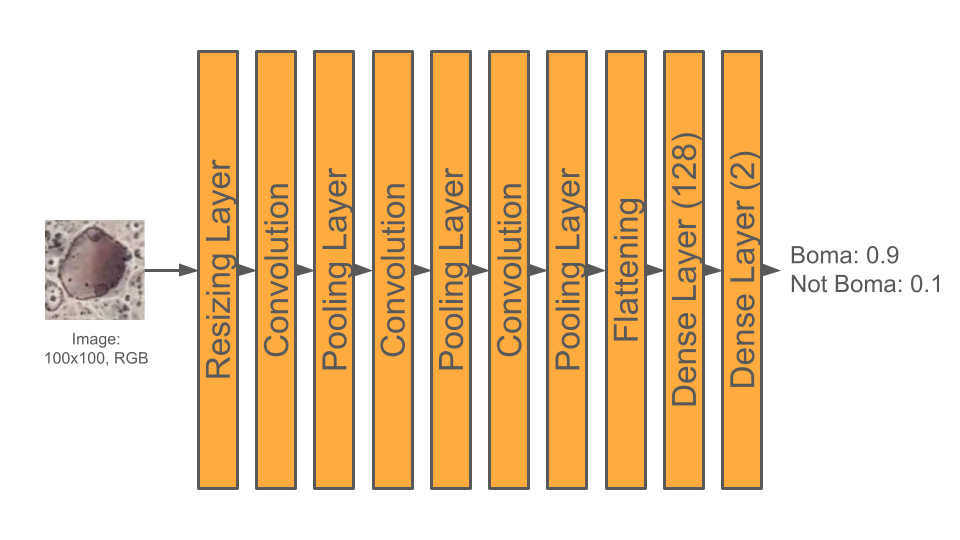
\includegraphics[width=1\linewidth]{images/Model Shape.png}
    \caption{Schematic of the Model}
    \label{fig:model_shape}
\end{figure}

The model, in particular, is a generic CNN model that can classify objects with relatively minimal training. Here's a quick explanation of each layer's function in the model.

Resizing layer: Rescale all the image values between 0 and 1 to normalize all of the values. This is done to ensure that all features are within the same scale.

Convolutional Layers (Conv2d): it has three layers that apply filters to the image to highlight features like edges, textures, or patterns. In this case, it most likely filters for circular or closed shapes similar to the shape of the Boma.

MaxPooling Layers: After each Conv2d Layer, there's a pooling layer that reduces the size of the filtered image by only keeping the most prominent features in each small area. This makes the model faster and focuses on the most critical parts of the image.

Flattening Layer: After filtering and Pooling, the model flattens the data, turning the 2d filtered images into a long list of numbers. This prepares the data for the final classification.

Dense Layer: There are two dense layers. It takes the flattened Layer and transforms it through another ReLU layer, reducing it to a 128-dimensional vector. This helps in capturing relationships between filtered features. Dense layers output logits, the softmax function is usually added at the end to output probabilities, providing a probability to be classified as a Boma "P(A)"

Finally, the model takes the probability from the softmax function and outputs them into a final set of 2 scores: probability it is a Boma "P(A)" and probability it isn't a Boma "1-P(A)".

\subsection{Model Testing}

\begin{figure} [H]
    \centering
    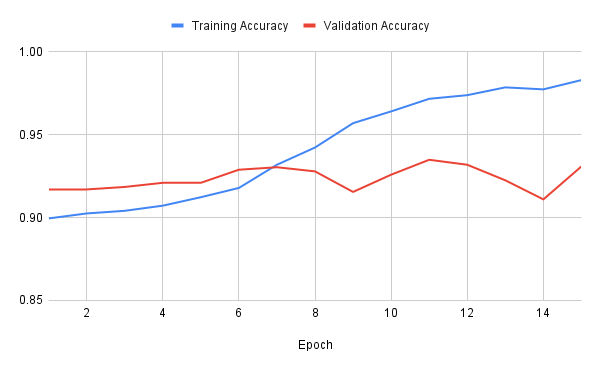
\includegraphics[width=1\linewidth]{images/Training Accuracy.png}
    \caption{Accuracy over 15 epochs}
    \label{fig:Accuracy_Chart}
\end{figure}

After Training the first time with 15 epochs, the accuracy plateaus around 97\% (Fig.~\ref{fig:Accuracy_Chart}). Therefore, for future training, the model was limited to 10 epochs. Additionally, Training Loss minimizes around 12-14 epochs (Fig.~\ref{fig:Loss_Chart}).

% \begin{table} [H]
%     \centering
%     \begin{tabular}{rrrl}
%     \multicolumn{1}{c}{\textbf{Epoch}} & \multicolumn{1}{c}{\textbf{Training Loss}} & \multicolumn{1}{c}{\textbf{Training Accuracy}} &  \\
%     1  & 0.3279 & 0.8995 &  \\
%     2  & 0.3031 & 0.9025 &  \\
%     3  & 0.2801 & 0.9041 &  \\
%     4  & 0.2526 & 0.9072 &  \\
%     5  & 0.2267 & 0.9123 &  \\
%     6  & 0.1942 & 0.9179 &  \\
%     7  & 0.1612 & 0.9319 &  \\
%     8  & 0.1353 & 0.9423 &  \\
%     9  & 0.1091 & 0.957  &  \\
%     10 & 0.091  & 0.9641 &  \\
%     11 & 0.075  & 0.9717 &  \\
%     12 & 0.0653 & 0.9739 &  \\
%     13 & 0.0543 & 0.9786 &  \\
%     14 & 0.0546 & 0.9774 &  \\
%     15 & 0.044  & 0.983  & 
%     \end{tabular}
%     \caption{Raw data from Training for 15 epochs}
%     \label{tab:training_raw_data}
% \end{table}

\begin{figure} [H]
    \centering
    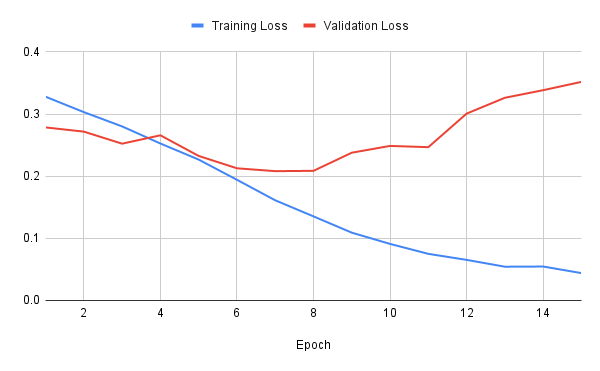
\includegraphics[width=1\linewidth]{images/Training Loss.png}
    \caption{Loss over 15 Epochs}
    \label{fig:Loss_Chart}
\end{figure}


% ------------------------------------------------------------------------------------

\subsection{Spatial Coordinate Extraction}
\label{procedure}
% Deploying the model?

Google Earth Engine (GEE) enables an image processing technique called "Image Stacking." Typically, These stacks would allow users to perform time-series analysis, detect trends, and monitor environmental changes using satellite imagery and other geospatial data. However, there is a lesser-known technique in which the user "squashes" the highest-resolution sections together to generate exceptionally high-resolution content to read. This can be useful, especially for filling holes in scanning, removing lower-resolution mapping, or avoiding cloudy content. 

A specified sample of the Monduli district of just over 260 square miles was chosen (Fig~\ref{fig:designated_area}) and 
 it was isolated for recent times in the last four weeks (2024-02-01 to 2024-02-29). The images were manually isolated with no cloud coverage over the selection area.

\begin{figure} [H]
    \centering
    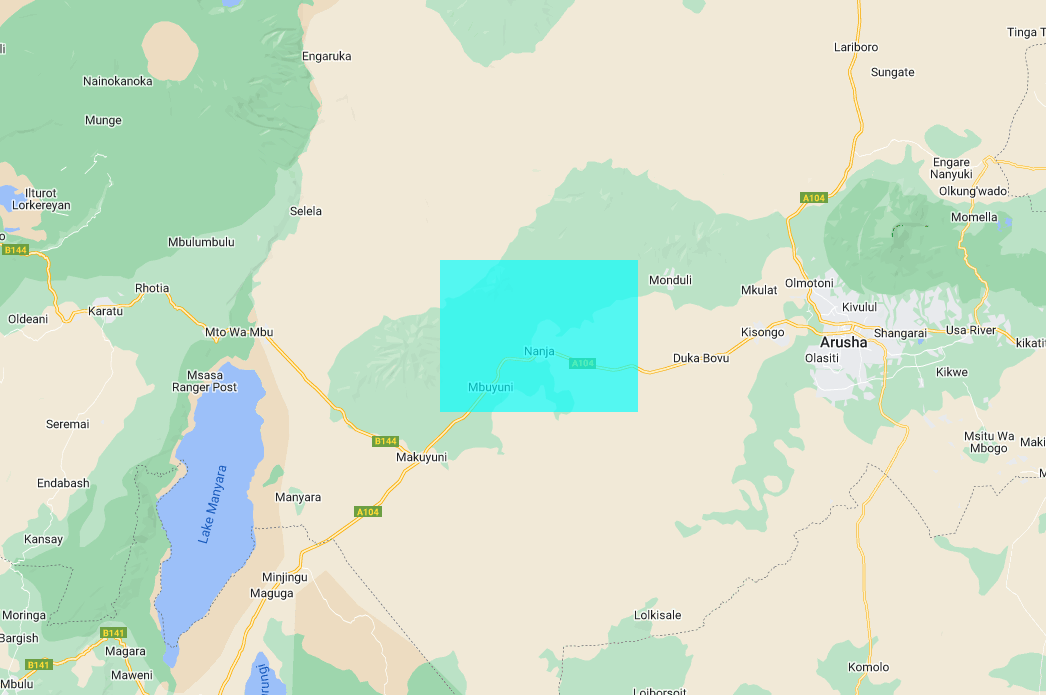
\includegraphics[width=1\linewidth]{images/studyarea.png}
    \caption{Designated Area for First Test, 260 square miles between Serengeti and Arusha}
    \label{fig:designated_area}
\end{figure}

All bands greater than 10-20 meters per pixel were filtered out of the image stack. For Copernicus/S2\_Harmonized, those included ['B2', 'B3', 'B4', 'B5', 'B6', 'B7', 'B8', 'B8A', 'B11', 'B12'] (Fig~\ref{fig:cop_bands_chart}). Then, the images were layered according to the variable importance GEE provided (Fig~\ref{fig:band_importance}). An image stack was created of all collected wavelengths of color light.

\begin{figure} [H]
    \centering
    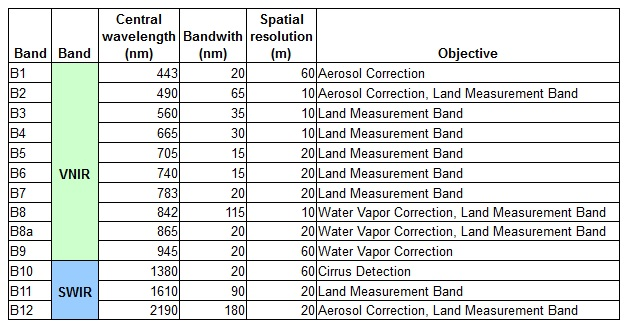
\includegraphics[width=1\linewidth]{images/copernicus_band_resolution.png}
    \caption{Band Resolutions Provided by Copernicus}
    \label{fig:cop_bands_chart}
\end{figure}

\begin{figure} [H]
    \centering
    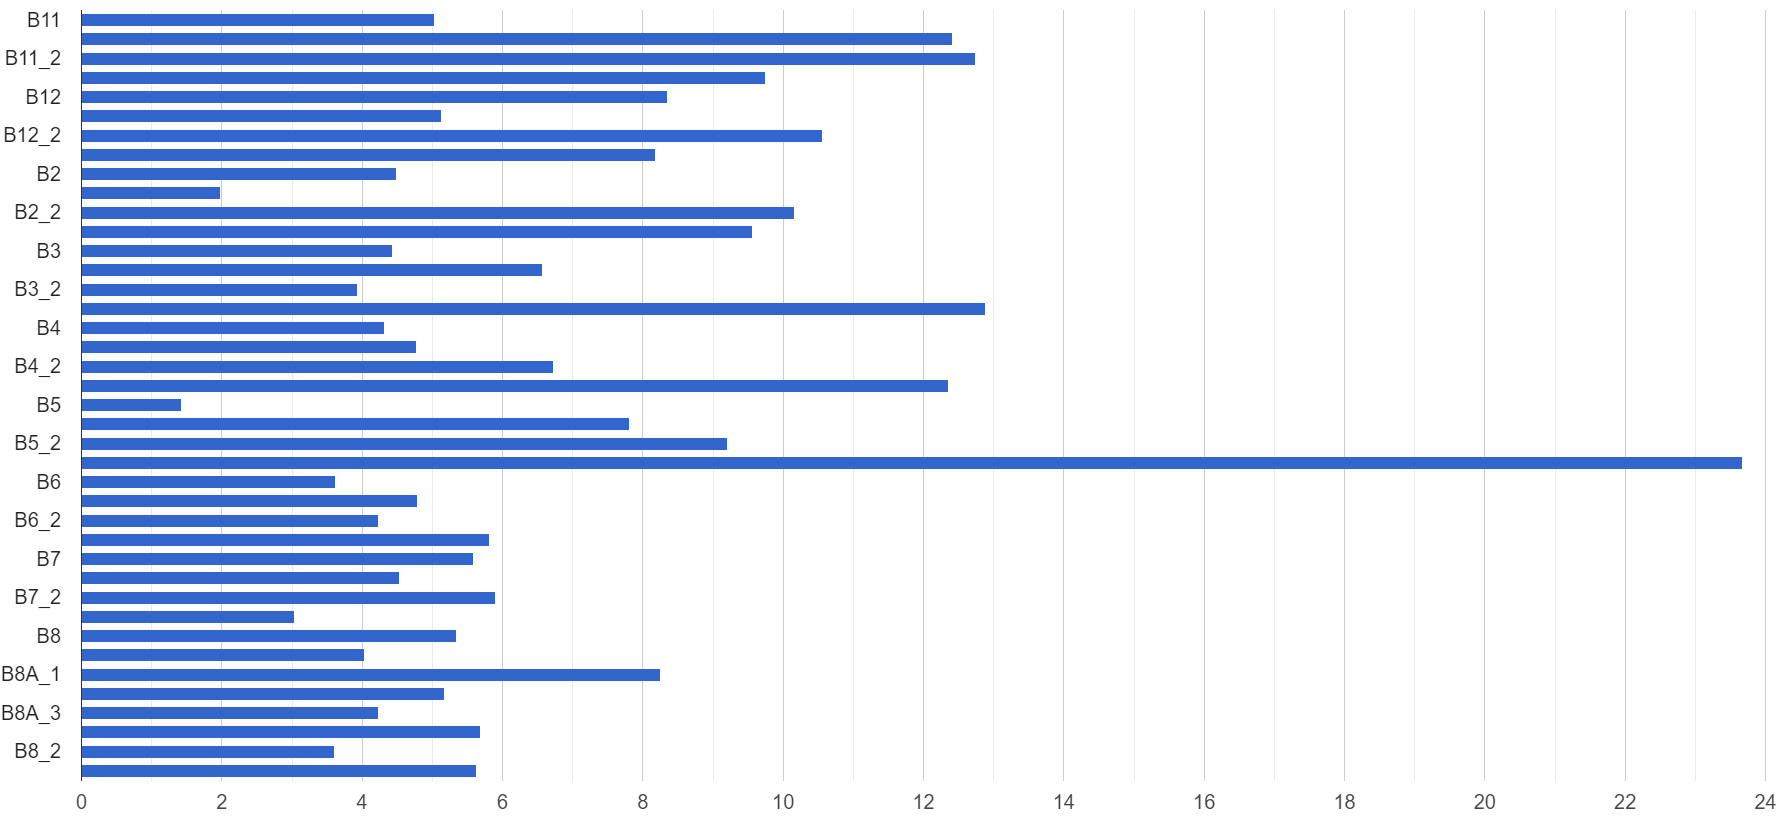
\includegraphics[width=1\linewidth]{images/bands importance.png}
    \caption{Variable Band Priority}
    \label{fig:band_importance}
\end{figure}

The image stack was seperated into slices run individually through the model (Fig~\ref{fig:model_shape}). The final image stack was 10980 pixels by 10980 pixels. To classify some of these Bomas accurately, the samples overlapped by a 20-pixel overlap in both the horizontal and vertical directions for edge cases where a Boma would be too far into the border and missed by either selection.

% ------------------------------------------------------------------------------------

\section{Results}
% Green Dot converted into heatmap; Black small dots
% Discussion for location of water bodies/water harvesting units

It took over 4 hours to run the model discussed in section~\ref{training} over the selected area of 260 square miles on GEE. Everywhere the confidence of the model was above 80\%, the coordinates of that point were recorded (Fig~\ref{fig:OutputOnSample}). Figure~\ref{fig:OutputOnSample} displays a dot for each recorded sample plotted out by relative coordinate. In total, the model classified 488 Bomas over the selected area. The relative coordinates were transposed on top of the image stack of the designated area generated in section~\ref{procedure} (Fig~\ref{fig:OverlayedMap}). Figure~\ref{fig:OverlayedMap} displays all the classified Bomas relative to Nanja Dam (natural reservoir).

\begin{figure} [H]
    \centering
    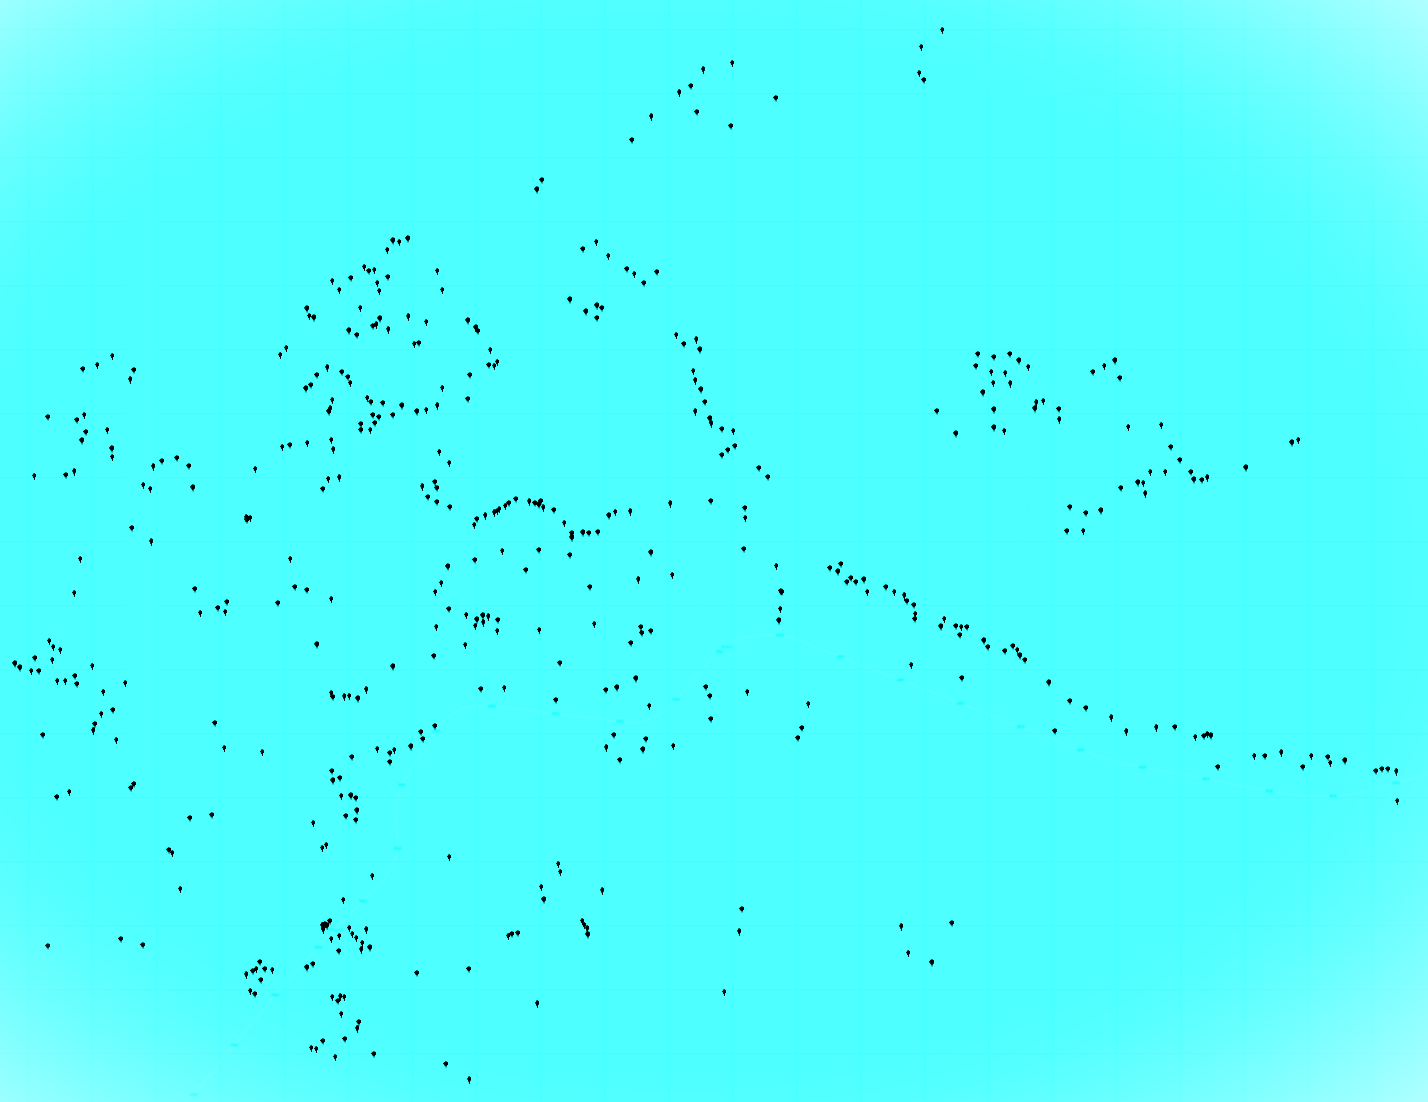
\includegraphics[width=1\linewidth]{images/cv_output.png}
    \caption{Output with relative coordinates}
    \label{fig:OutputOnSample}
\end{figure}

\begin{figure} [H]
    \centering
    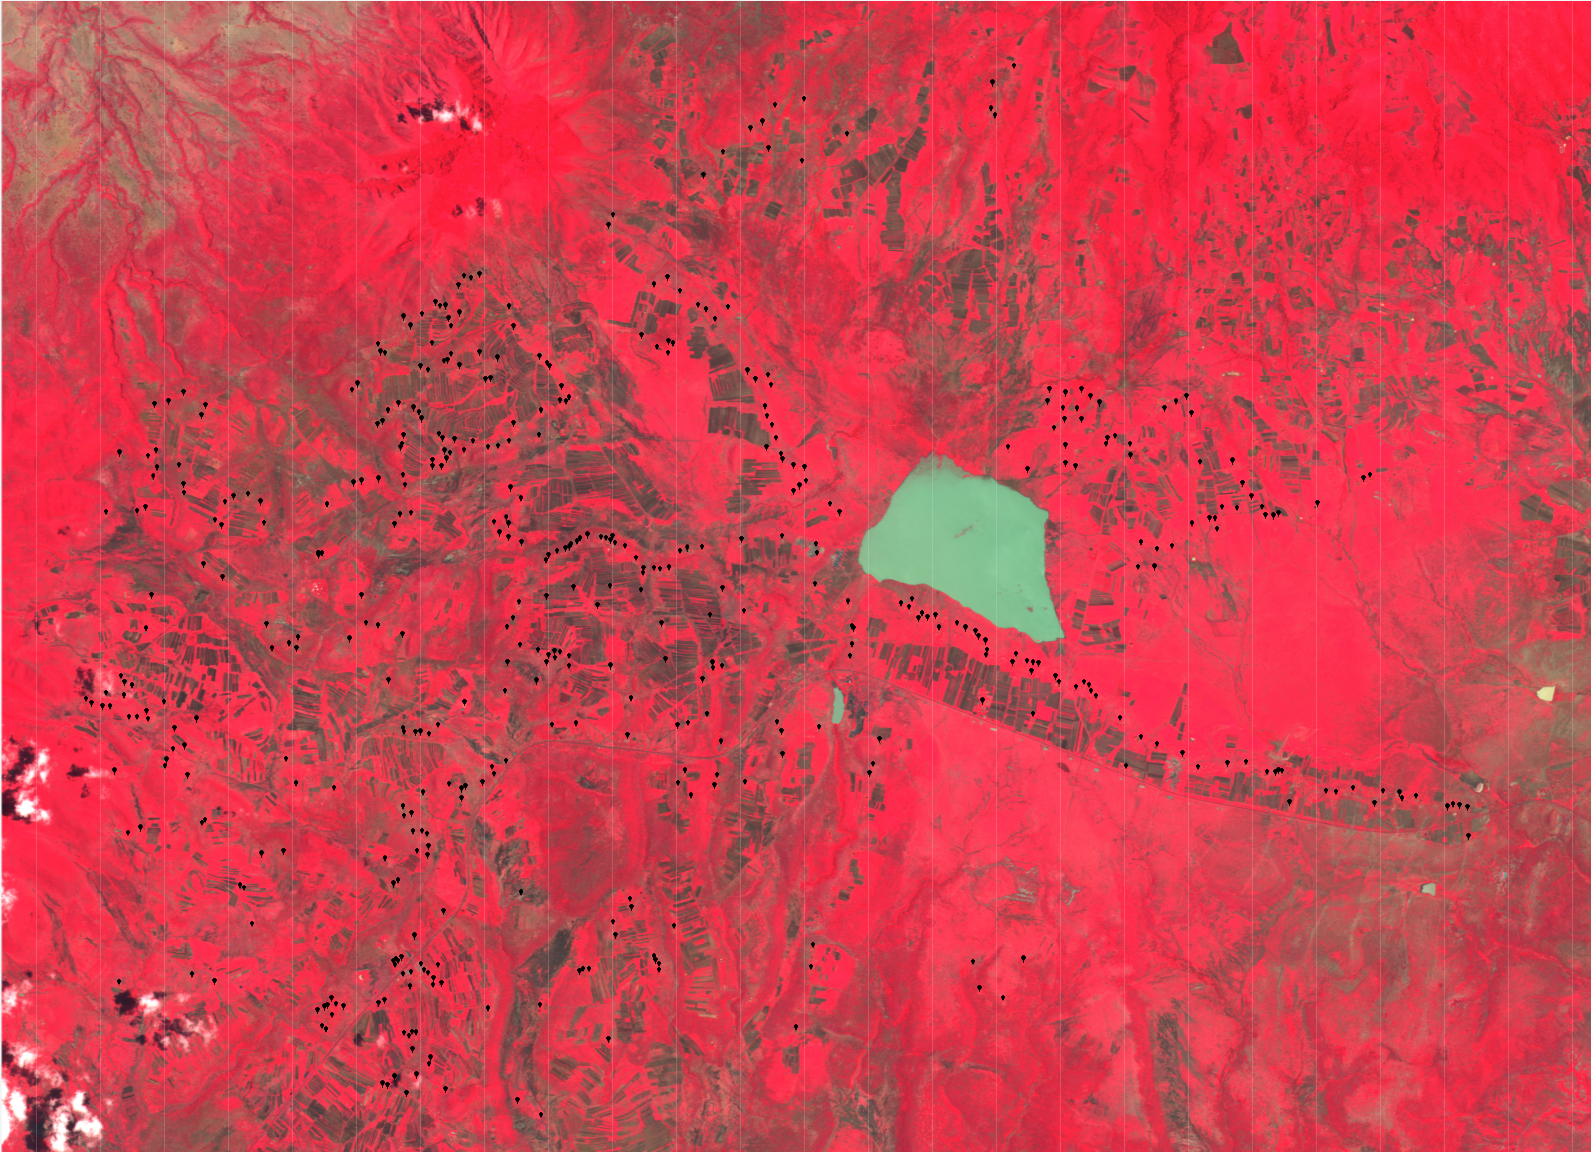
\includegraphics[width=1\linewidth]{images/Outputoverlayrealmap.png}
    \caption{Output Overlayed Over Image Stack}
    \label{fig:OverlayedMap}
\end{figure}

% ------------------------------------------------------------------------------------

\section{Discussion}

\subsection{Key Findings}

It is evident that large populations seem to live in dense communities of several dozen Bomas (A, B, F, J, K). They also live in lines along the edges of major geological formations such as dried riverbeds or reservoirs (C, E, G). In addition, it also looks like many communities reside parallel to the major highway that runs through the area (H, I). This information can be used to isolate large communities and identify the best locations for rainwater harvesting solutions (Fig~\ref{fig:Communities and Major Highway}).

\begin{figure} [H]
    \centering
    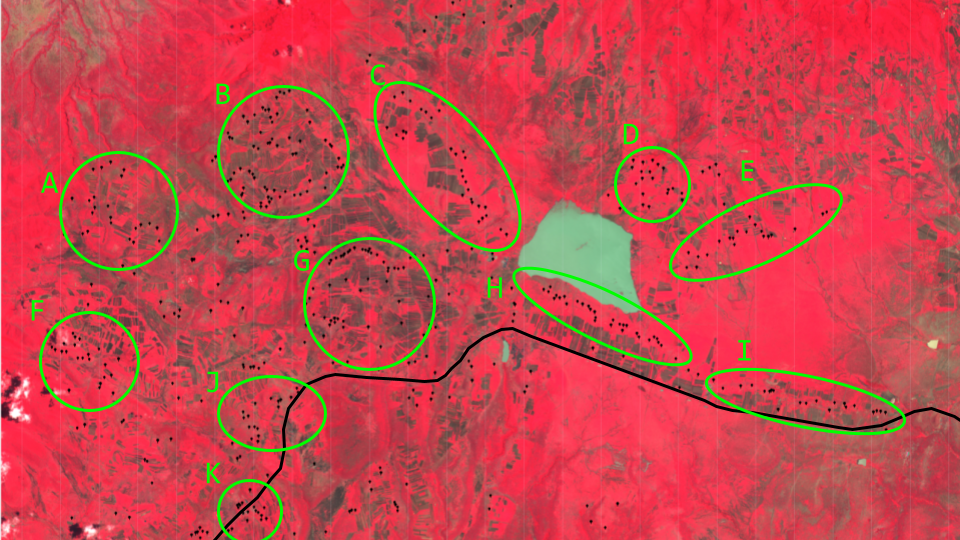
\includegraphics[width=1\linewidth]{images/Communities and Highway Highlighted.png}
    \caption{Large High-Density Community Collections of Bomas Highlighted with Major Highway}
    \label{fig:Communities and Major Highway}
\end{figure}

Larger groups, especially those further away from the Nanja Dam, such as A, B, and F, are this project's starting point, and identifying locations within these more prominent groups to place these water harvesting solutions is the next step. 

\subsection{Limitations of Outputs}

As you can see in the zoomed-in photos, the images streamed to the web editor are very low quality from the perspective of the GEE editor. However, there are noticeable patterns where the model "identified" Bomas (Fig~\ref{fig:Zoomed_Overlayed}). A quick look at the coordinates in Google Maps (with higher resolution but dated images) shows that at least a couple of these points seem to be housing units. However, many Bomas seem not identified (Fig~\ref{fig:zoomed_google_maps}), or only large, easily identifiable with thick or dark boundaries are identified.

\begin{figure} [H]
    \centering
    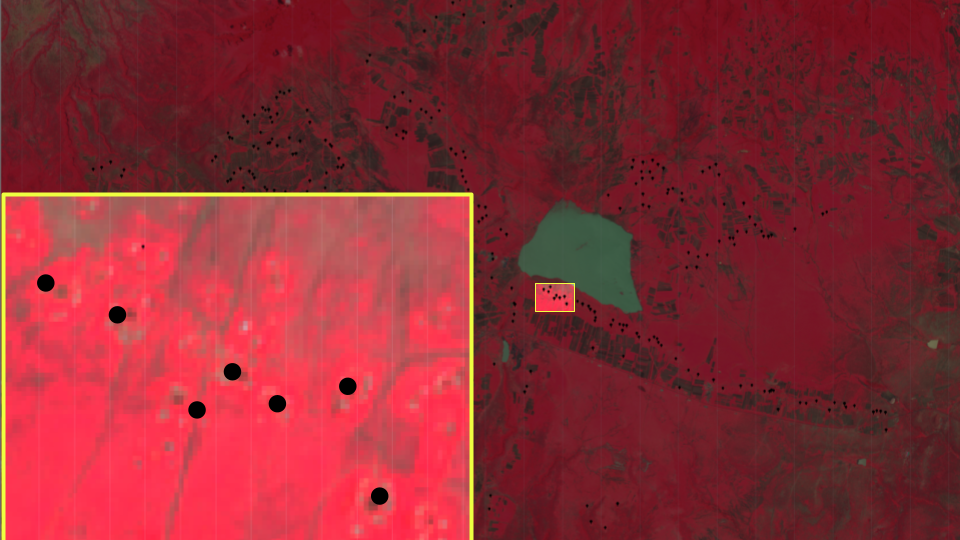
\includegraphics[width=1\linewidth]{images/zoomed in overlay.png}
    \caption{Zoomed In Portion on GEE}
    \label{fig:Zoomed_Overlayed}
\end{figure}

\begin{figure} [H]
    \centering
    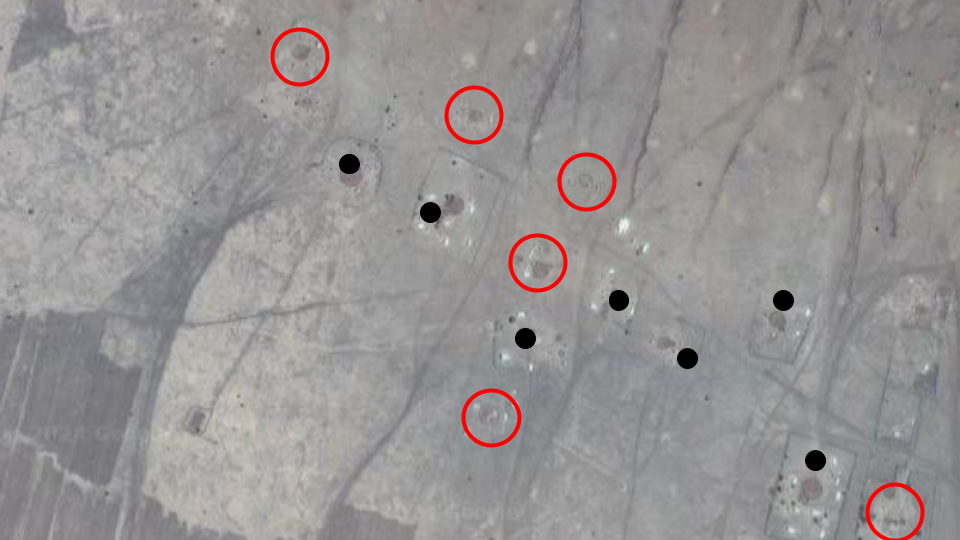
\includegraphics[width=1\linewidth]{images/zoomed google maps highlighted.png}
    \caption{Zoomed In Portion on Google Maps Displaying False Negatives}
    \label{fig:zoomed_google_maps}
\end{figure}

In addition, the training data may have caused some of these inaccuracies. The dataset was very unbalanced, with 75\% of the data being photos of Bomas and only 25\% of the data being photos of the environment. The model may have been more accurate with a more balanced training set.

\subsection{Implications and Significance}

Maps like these can be used in numerous contexts, especially in other humanitarian efforts. Now that the population locations is better understood, the data can be used to structure other initiatives, like drone-based medical delivery, better road systems, or the locations of medical facilities. Other organizations, or even the Tanzanian Government, could use this data to understand better where their Indigenous populations are located.

\subsection{Community Involvement}

The outputs' results are being validated with local Maasai community (a formal group of Maasai members from across the region). With the validated data, the next step is to segment the map into high-density, medium-density, and low-density clusters. Identifying the best possible water access solutions is based on the size and area of the clusters.

Three types of deployment solutions are being evaluated with the community. The first is a low-cost solution of 5000-liter tanks with rainwater harvesting at a Boma. This applies to distant Bomas, which are not close to any significant water access location. The second is a sizeable 100,000-liter water harvesting solution deployed for a set of Bomas together that will be helpful for large-density/medium-density regions. The third is a man-made pond/small lake where rainwater collects, and a solar-powered pump and filtration unit provide clean water access.

One of the core principles of ensuring long-term sustained impact and ownership is to empower and enable the local Maasai community to pick these solutions and invest their time in the planning, deployment, and ongoing maintenance. With over 480+ Bomas and 50000 Maasai, establishing a more structured Water Council that takes accountability for equitable water use and ongoing maintenance will be crucial. This work is done with Maji Wells [Mbayani Tayai, local Maasai leader] and other local community leads.

% ------------------------------------------------------------------------------------

\section{Conclusion}

This study has demonstrated the potential of integrating advanced satellite imagery analysis with traditional water management practices to significantly enhance water accessibility for the Maasai communities in Northern Tanzania. By employing TensorFlow in conjunction with Google Earth Engine, a model was developed that identifies populations. These maps can optimize water solution placement, tailoring solutions to the region's unique geographical and social structure.

A mix of individual and communal rainwater harvesting units are being built in or near the locations.

Future efforts should focus on refining the models' predictive accuracy by in corporating more diverse data sets and real-time environmental monitoring. Additionally, exploring partnerships with local governments and international organizations will be crucial in scaling these solutions to other similarly affected communities globally. By continuously blending technology with traditional knowledge, more resilient communities can be better equipped to manage their natural resources sustainably.

\section*{Acknowledgement}

We thank Ananya Rao (Carnegie Mellon University) for mentoring and supporting this project and Mbayani Tayai for validating ground truths in Tanzania.

\printbibliography

\end{document}